\documentclass[border=6pt]{standalone}
\usepackage{amsmath}
\usepackage{amssymb}
\usepackage{tikz}
\usepackage{pgfplots}
\pgfplotsset{compat=1.18}
\usetikzlibrary{arrows.meta,calc,positioning}
\begin{document}
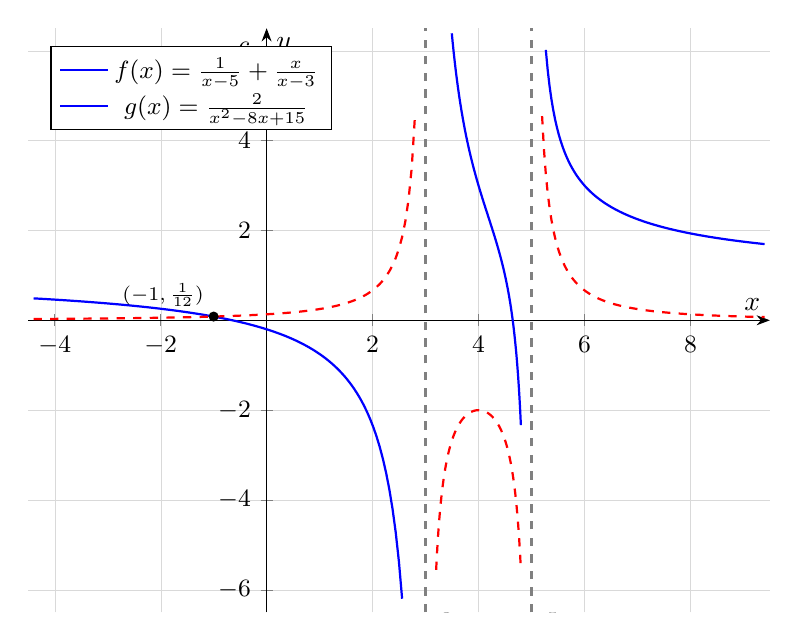
\begin{tikzpicture}
\begin{axis}[
    axis lines = middle,
    xlabel = {$x$}, ylabel = {$y$},
    grid=both,
    grid style={line width=.1pt, draw=gray!30},
    axis line style={-Stealth},
    legend style={font=\small},
    tick label style={font=\small},
    xmin=-4.5, xmax=9.5, ymin=-6.5, ymax=6.5,
    xtick={-4,-2,0,2,4,6,8},
    ytick={-6,-4,-2,0,2,4,6},
    width=11cm, height=9cm,
    legend pos=north west,
]
\addplot[domain=-4.4:2.8, samples=120, restrict y to domain=-6.5:6.5, thick, blue] {1/(x-5) + x/(x-3)};
\addplot[domain=3.2:4.8, samples=120, restrict y to domain=-6.5:6.5, thick, blue] {1/(x-5) + x/(x-3)};
\addplot[domain=5.2:9.4, samples=120, restrict y to domain=-6.5:6.5, thick, blue] {1/(x-5) + x/(x-3)};
\addlegendentry{$f(x)=\frac{1}{x-5}+\frac{x}{x-3}$}
\addplot[domain=-4.4:2.8, samples=120, restrict y to domain=-6.5:6.5, thick, red, dashed] {2/((x-5)*(x-3))};
\addplot[domain=3.2:4.8, samples=120, restrict y to domain=-6.5:6.5, thick, red, dashed] {2/((x-5)*(x-3))};
\addplot[domain=5.2:9.4, samples=120, restrict y to domain=-6.5:6.5, thick, red, dashed] {2/((x-5)*(x-3))};
\addlegendentry{$g(x)=\frac{2}{x^2-8x+15}$}
\draw[dashed, gray, thick] (axis cs:3,-6.5) -- (axis cs:3,6.5);
\draw[dashed, gray, thick] (axis cs:5,-6.5) -- (axis cs:5,6.5);
\node[anchor=north, font=\scriptsize, gray] at (axis cs:3,-6.3) {$x=3$};
\node[anchor=north, font=\scriptsize, gray] at (axis cs:5,-6.3) {$x=5$};
\addplot[only marks, mark=*, mark size=1.6pt, black] coordinates {(-1,0.0833)};
\node[anchor=south east, font=\scriptsize] at (axis cs:-1,0.0833) {$(-1,\tfrac{1}{12})$};
\end{axis}
\end{tikzpicture}
\end{document}
